\begin{scanpage}{0073}{56}
\begin{center}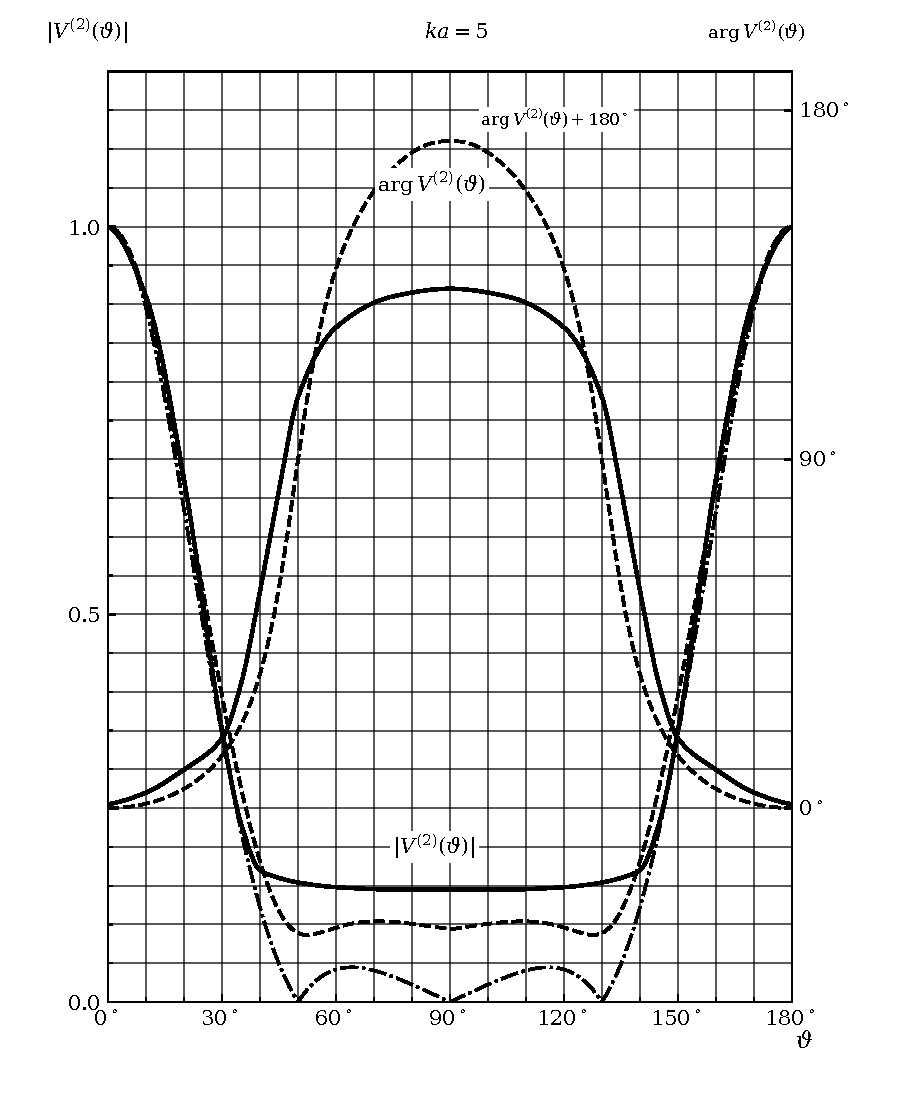
\includegraphics[height=11cm]{images/recreated/a-0073-fig21.pdf}\par Figure 21. The function $V^{(2)}(\theta)$ for a disk with normal incidence of a plane wave. The various curves correspond to different approximations.\end{center}
and in the case of H-polarization $(\mathbf H_0\perp yoz)$
\[\left.\begin{aligned}E_\theta=H_\phi&=-iaH_{0x}\cos\theta\sin\phi\frac{J_1(ka\sqrt{\lambda^2+\mu^2})}{\sqrt{\lambda^2+\mu^2}}\frac{e^{ikR}}R,\\E_\phi=-H_\theta&=-iaH_{0x}\cos\phi\frac{J_1(ka\sqrt{\lambda^2+\mu^2})}{\sqrt{\lambda^2+\mu^2}}\frac{e^{ikR}}R.\end{aligned}\right\}\tag{10.04}\]
The quantities $\lambda$ and $\mu$ in Equations (10.03) and (10.04) are determined in the following way:
\[\left.\begin{aligned}\lambda&=\sin\theta\cos\phi,\\\mu&=\sin\theta\sin\phi-\sin\gamma,\\\sqrt{\lambda^2+\mu^2}&\geq0.\end{aligned}\right\}\tag{10.05}\]
\end{scanpage}
